% =============================================================================
%  COMPONENT COOKBOOK  --  not part of your deck
%  ---------------------------------------------------------------------------
%  Copy a frame from this file into Sections/ and adapt it.
%  To preview every component in Overleaf: set this file as the main document,
%  compile, then switch back to main.tex.
% =============================================================================
\documentclass[10pt, aspectratio=169]{beamer}

\usepackage{Preamble/preamble}
% =============================================================================
%  BRANDING  --  edit the four lines below and the whole deck follows.
% =============================================================================
\definecolor{BrandPrimary}{RGB}{36, 164, 220}   % main colour (bars, section dividers)
\definecolor{BrandAccent}{RGB}{201, 42, 135}    % accent (alerts, highlights)
\definecolor{BrandDark}{RGB}{0, 33, 71}         % dark text / contrast
\newcommand{\brandlogo}{Assets/logo.png}        % empty {} to hide the logo
% =============================================================================

% --- Beamer colours ---------------------------------------------------------
\setbeamercolor{palette primary}{bg=BrandPrimary, fg=white}
\setbeamercolor{structure}{fg=BrandPrimary}
\setbeamercolor{titlelike}{fg=BrandPrimary}
\setbeamercolor{frametitle}{bg=BrandPrimary, fg=white}
\setbeamercolor{alerted text}{fg=BrandAccent}
\setbeamercolor{block title}{bg=BrandPrimary!15, fg=BrandDark}
\setbeamercolor{block body}{bg=BrandPrimary!5}

% --- Links ------------------------------------------------------------------
% Deferred to \begin{document} so hyperref is guaranteed to be loaded already.
\AtBeginDocument{%
  \hypersetup{
    colorlinks=true,
    linkcolor=BrandPrimary,
    urlcolor=BrandPrimary,
    citecolor=BrandPrimary
  }%
}


\title{Component Cookbook}
\author{Beamer Template}
\institute{Preview only -- copy what you need}
\date{\today}

\begin{document}

% =============================================================================
%  1. TWO COLUMNS: TEXT + IMAGE
% =============================================================================
\begin{frame}{Two columns: text and image}
    \begin{columns}[T, onlytextwidth]
        \begin{column}{0.55\textwidth}
            \begin{itemize}
                \item Keep each column to three or four short points
                \item Use \texttt{onlytextwidth} so the outer margins stay intact
                \item Swap the widths (0.55 / 0.42) to shift emphasis
            \end{itemize}
        \end{column}
        \begin{column}{0.42\textwidth}
            \centering
            % \includegraphics[width=\linewidth]{Assets/your-image.png}
            
\begin{tikzpicture}
                \node[draw=BrandPrimary, fill=BrandPrimary!10, rounded corners,
                      minimum width=4cm, minimum height=3.4cm, align=center,
                      text=BrandPrimary] {Your image\\goes here};
            \end{tikzpicture}
        \end{column}
    \end{columns}
\end{frame}

% =============================================================================
%  2. FULL-WIDTH FIGURE WITH CAPTION
% =============================================================================
\begin{frame}{Full-width figure}
    \begin{figure}
        \centering
        % \includegraphics[width=0.8\linewidth]{Assets/your-image.png}
        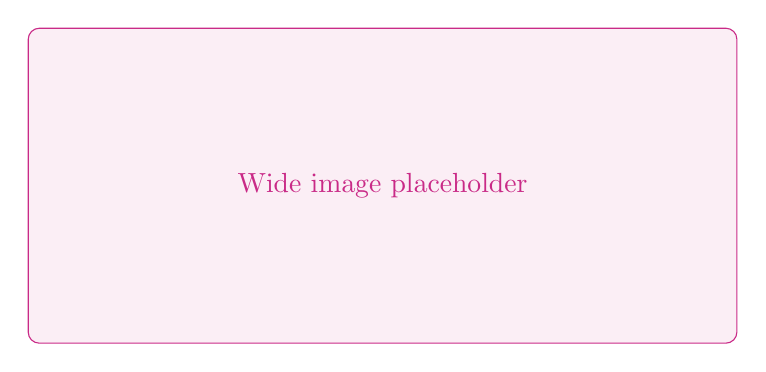
\begin{tikzpicture}
            \node[draw=BrandAccent, fill=BrandAccent!8, rounded corners,
                  minimum width=9cm, minimum height=4cm, align=center,
                  text=BrandAccent] {Wide image placeholder};
        \end{tikzpicture}
        \caption{Always say what the figure shows, not that it is a figure.}
    \end{figure}
\end{frame}

% =============================================================================
%  3. TABLE (booktabs)
% =============================================================================
\begin{frame}{Table}
    \centering
    \begin{tabular}{lrr}
        \toprule
        \textbf{Item} & \textbf{2025} & \textbf{2026} \\
        \midrule
        Revenue        & 1\,200 & 1\,480 \\
        Operating cost & 740    & 810    \\
        Margin         & 460    & 670    \\
        \bottomrule
    \end{tabular}

    \vspace{0.6cm}
    {\small Tables stay readable when they have no vertical rules.}
\end{frame}

% =============================================================================
%  4. CALLOUT BOXES
% =============================================================================
\begin{frame}{Callout boxes}
    \begin{tcolorbox}[colback=BrandPrimary!8, colframe=BrandPrimary,
                      boxrule=0.6pt, arc=3pt, title=Definition]
        A short statement of the concept being introduced.
    \end{tcolorbox}

    \vspace{0.2cm}

    \begin{tcolorbox}[colback=BrandAccent!8, colframe=BrandAccent,
                      boxrule=0.6pt, arc=3pt, title=Warning]
        Something the audience should not misunderstand.
    \end{tcolorbox}
\end{frame}

% =============================================================================
%  5. TIKZ FLOW DIAGRAM
% =============================================================================
\begin{frame}{Flow diagram}
    \centering
    \begin{tikzpicture}[
        node distance=6mm,
        box/.style={rectangle, rounded corners, draw=BrandPrimary, thick,
                    fill=BrandPrimary!8, minimum width=2.6cm, minimum height=0.9cm,
                    align=center, font=\small\bfseries},
        arrow/.style={-{Stealth}, thick, draw=BrandDark}
    ]
        \node[box] (a) {Input};
        \node[box, right=of a] (b) {Process};
        \node[box, right=of b] (c) {Output};
        \draw[arrow] (a) -- (b);
        \draw[arrow] (b) -- (c);
    \end{tikzpicture}
\end{frame}

% =============================================================================
%  6. CODE LISTING  --  the frame MUST be [fragile]
% =============================================================================
\begin{frame}[fragile]{Code listing}
    \begin{lstlisting}[language=Python, caption={Minimal example}]
def greet(name):
    """Return a greeting."""
    return f"Hello, {name}!"
    \end{lstlisting}
\end{frame}

% =============================================================================
%  7. BLOCKS
% =============================================================================
\begin{frame}{Blocks}
    \begin{block}{Standard block}
        Default block, inherits the brand palette.
    \end{block}

    \begin{alertblock}{Alert block}
        Use for risks, errors or anything that needs attention.
    \end{alertblock}

    \begin{exampleblock}{Example block}
        Use for worked examples.
    \end{exampleblock}
\end{frame}

% =============================================================================
%  8. STATEMENT SLIDE  --  one sentence, maximum impact
% =============================================================================
\begin{frame}[plain]
    \centering
    \vfill
    {\Huge\bfseries\color{BrandPrimary}
     One idea per slide.\\[0.3cm]
     Say it in one sentence.}
    \vfill
\end{frame}

% =============================================================================
%  9. QUOTE
% =============================================================================
\begin{frame}{Quote}
    \vspace{1cm}
    \begin{quote}
        \large\itshape
        ``Quote the source, not your memory of it.''\\[0.4cm]
        \normalsize\upshape --- Author, \textit{Source} (Year)
    \end{quote}
\end{frame}

% =============================================================================
%  10. CLOSING SLIDE
% =============================================================================
\begin{frame}[plain]
    \centering
    \vfill
    {\Huge\bfseries\color{BrandPrimary} Thank you}\\[0.4cm]
    {\Large Questions \& Discussion}
    \vfill
    \IfFileExists{\brandlogo}{%
        \includegraphics[height=1.2cm, keepaspectratio]{\brandlogo}%
    }{}
    \vspace{0.5cm}
\end{frame}

\end{document}
